\documentclass{article} 

% the purpose of this particular document is to serve as a staging area potential blog posts, for the purpose of editing, revision, and review. 

% packages 
	\usepackage{amsmath, amsthm, mathtools}
	\usepackage{mdframed}  
	\usepackage{geometry, enumerate} 
	\usepackage{parskip}
	\usepackage{graphicx}

% theorems and such 
  	\newtheorem{theorem}{Theorem}
  	\newtheorem{corollary}{Corollary}
  	\newtheorem{lemma}[theorem]{Lemma} 
  	\newtheorem*{remark}{Remark}
  	\newtheorem*{exe}{Exercise}
  	\newtheorem{prop}{Proposition} 
  	
% custom commands 
	\newcommand{\ceil}[1]{\left \lceil #1 \right \rceil}
	\newcommand{\floor}[1]{\lfloor #1 \rfloor}
	\newcommand{\X}[1]{\, \text{mod} \, #1}
	\newcommand{\divv}{\,|\,}
	\newcommand{\GCD}[2]{GCD\,(#1, #2)}
	\newcommand{\LCM}[2]{LCM\,(#1, #2)}

\begin{document} 

\title{Elementary Number Theory : \S 1} 
\author{Henry Slayer $|$ University of California, Santa Cruz} 
\date{}
\maketitle

\section*{The Euclidean Algorithm} 
The first scientific study of the numbers is typically attributed to the Greeks, who began classifying and categorizing the numbers (odd, even, etc…) in around 600 BC. It is Euclid, however, who transformed the theory of numbers into a deductive science. His \textit{Elements} was truly a master work of geometry and number theory, and in Book VII, the Euclidean Algorithm was born. Euclid's algorithm is an iterated process of division with remainder on two positive integers. Though simple, it is the foundation upon which much of number theory stands. For more on the \textit{Elements}, David Joyce has an interactive (albeit dated) browser version of the text, with Java applets to boot. 
\begin{verbatim} https://mathcs.clarku.edu/~djoyce/java/elements/elements.html 
\end{verbatim} 

For what follows, we’ll take a leaf out of Weissman’s book, and start by exploring the dynamic nature of numbers in pairs. In other words, if we treat numbers as moves or units of measure, where can we go? What can we scale? The answer will lead us right into the hands of Euclid’s numerical disassembly.  
\subsubsection*{Compound Moves} 
The dynamic interpretation of division with remainder is best served by an example. Suppose we have two measuring sticks, one that measures 61 units, and another that measures 39 units. Using only these two rulers, what can we measure? All multiples of 39 and 61, surely, but we can do better. How? We build a new measuring stick out of our first two. Lining up the two side-by-side, we can measure out a new ruler, from the difference, which is 61 - 39 = 22 units long. Nice! Now, we can measure anything that’s 61, 39, or 22 units long. What if we did it again? Taking the smaller of our two original numbers, we could use the difference of the 39-unit rule and the 22-unit rule to measure out lengths of 17. 

\begin{figure}[h!]
%\begin{mdframed} 
	\center{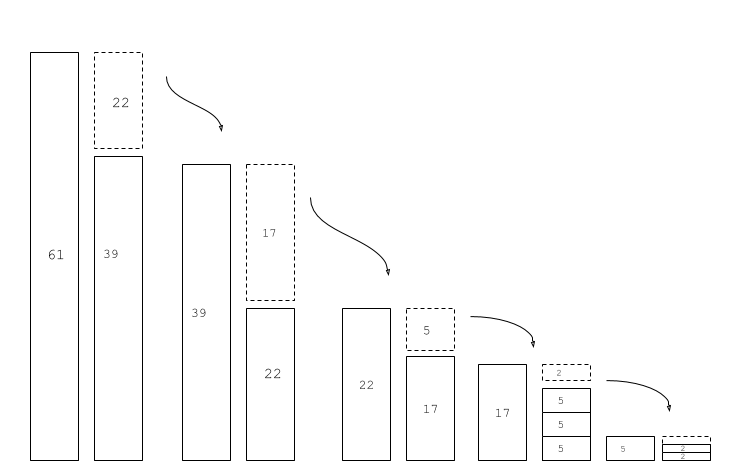
\includegraphics[width=.8\textwidth]
		{figEA.png}}
%\end{mdframed} 
\end{figure}
And again, taking the 22 unit rule and the 17 unit rule, we get down to a precision of 5. If we take 3 of our new 5-unit rulers, we can compare the three stacked together to the 17 unit rule and measure lengths of 2. Taking two of the two unit rules with 5 gets us down to a single unit. Scaling our single-unit ruler allows us to measure anything that we want.  

Fundamentally, the Euclidean algorithm is no different. It is an iterative process of division with remainder. The steps that we took above are the same steps as the Euclidean algorithm, just written down a bit differently. In fact, if we wanted to formalize our process above, we would write
\begin{align*} 
	61 &= 1(39) + 22\\
	39 &= 1(22) + 17 \\
	22 &= 1(17) + 5 \\
	17 &= 3(5) + 2 \\
	5 &= 2(2) + 1
\end{align*} 

\subsubsection*{The Euclidean Algorithm} 

The Euclidean algorithm starts with two positive integers, $a$ and $b$. Assuming $a > b$, our first line step is to break down $a$ using division with remainder.  
\[a = q(b) + r\] 
Where $r$ is a whole remainder, and $0 \leq r < b$. The only rule that we follow, for now, is that $r$ is the least possible remainder. (The Euclidean algorithm actually comes in two flavors, as we’ll see, but for now, we assume that our remainders are whole, positive numbers). 
Then, we swap. The divisor ($b$) becomes the dividend (formerly $a$), and we divide our new divisor by the previous remainder. 
That can be a little tricky in words, but it’s swingin’ in practice. 
In equations: 

\begin{align*} 
a &= q_1(b) + r_1 \\
b &= q_2(r_1) + r_2 \\
r_1 &= q_3(r_2) + r_3)\\
&\vdots \\
r_{f-2} &= q_{f}(r_{f-1}) + r_f \\
r_{f-1} &= q_{f+1}(r_f) + 0  
\end{align*} 

When the remainder is zero (and we always reach zero because of the well-ordering principle) the process is over, and we stop. 

% provide another example here… maybe one with small numbers and one with large numbers  

\subsubsection*{The Euclidean Algorithm and the GCD} 

The Euclidean Algorithm is a powerful tool for systematically obtaining the greatest common divisor of two integers.
We mentioned the greatest common divisor last time, but to review, the GCD of two integers a and b is another number g with the following properties:
\begin{enumerate}[(i)] 
\item g is a common divisor of a and b 
\item if a and b have any other common divisors, those divisors also divide g 
\end{enumerate} 
We can make several observations about the greatest common divisor. 
\begin{mdframed} 
\begin{lemma} Let $a$ be an integer. Then 
\[GCD(a, 0) = a\]
\end{lemma}  
\begin{proof} Everything divides zero. That is to say, zero is a multiple of anything (we just multiply by zero). The greatest divisor of a is a itself. So, the greatest divisor of any integer a and 0 will be a itself. 
\end{proof}
\end{mdframed} 
\begin{mdframed} 
\begin{lemma}Suppose a, b, q, r are integers such that a = q(b) + r. Let g be another number. Then, g is the greatest common divisor of a and b if and only if g is the greatest common divisor of b and r.
\end{lemma} 
\begin{proof}
Fill in. 
\end{proof} 
\end{mdframed} 
These two lemmas tie the Euclidean algorithm to the greatest common divisor.
\begin{mdframed}
\begin{theorem}
Assume a and b are natural numbers, at least one of which is nonzero. Then, the final nonzero remainder produced by applying the Euclidean algorithm to a and b is the greatest common divisor of a and b. 
\end{theorem}
\begin{proof} In the terminal line of the euclidean algorithm, we see something of the sort 
\[a_n = q_n(b_n) + 0\] 
where $b_n$ is the final nonzero remainder. By what we’ve shown previously, $GCD(b_n, 0) = 0$. So, we walk up a line, which gives 
\[a_{n-1} = q_{n-1}(a_n) + b_n\]
Then, by the second lemma, the \(GCD(a_{n-1}, a_n) = GCD(a_n, b_n) = GCD(b_n, 0) = b_n\). 
Iterating this up our chain of divisions, we find that \(GCD(a, b) = \cdots = GCD(b_n, 0) = b_n\), the final nonzero remainder. 
\end{proof} 
\end{mdframed} 
\subsubsection*{GCD / LCM Product Formula} 

We’ll close by examining some of the properties of the greatest common divisor, as well as the least common multiple. 
The least common multiple ($LCM$) of two integers is another integer $l$, such that $l$ is a multiple of both $a$ and $b$ ($b\divv l$, $a\divv l$), such that any other multiple of $a$ and $b$ is larger. That is, if there exists some other multiple $m$, $l\divv m$. 

The greatest common divisor, the least common multiple, and the numbers that they’re defined by are all intimately related. 
\begin{mdframed} 
\begin{theorem} Let a and b be positive integers. Then 
	\[GCD(a, b) \cdot LCM(a, b) = ab\] 
\end{theorem} 
\begin{proof}  Let $GCD$ and $LCM$ denote the greatest common divisor and least common multiple, respectively, of a and b. The $GCD$ is a divisor of both $a$ and $b$, and the $LCM$ is a multiple of both $a$ and $b$, so 
\begin{align*} 
a = n\cdot GCD \quad&\quad b = m \cdot GCD \\  
LCM = x \cdot a \quad&\quad LCM = y \cdot b \\
\end{align*}
The $LCM$ is a multiple of $a$ and $b$, so it must be a multiple of $ab$ for some integer $g$. Similarly, we see that the $GCD$ of $a$ and $b$ is also a multiple of $ab$. So, with $g$ and $l$ as integers, 
\begin{align*}  
ab &= nm \cdot GCD = l \cdot GCD \\ 
ab &= LCM \cdot g 
\end{align*}
Using these  6 relations, we can deduce the following: 
\begin{align*}
ab = LCM \cdot g &= x \cdot a \cdot g  \quad \Rightarrow \quad  b = gx \\
ab = LCM \cdot g &= y \cdot b \cdot g  \quad \Rightarrow \quad  a = gy
\end{align*} 
So, $g\divv a$, $g\divv b$, and by definition, $g\divv GCD$. 
Secondly, we can observe that 
\[ab = l \cdot GCD \quad\Rightarrow am = l\] 
\[ab = l \cdot GCD \quad\Rightarrow  bn = l\] 
So, l is a common multiple of both a and b. By definition, then, $a\divv l$, $b\divv l$, and $LCM\divv l$. 
Now, we can assemble a tower of divisibilities.
\begin{enumerate}[] 
\item $a = g \cdot LCM$ and $g\divv GCD$, so, $a = (g \cdot LCM) \divv (GCD \cdot LCM)$  
\item Similarly, the $LCM\divv l$ as $l$ is a common multiple of $a$ and $b$, and $GCD\cdot l = ab$
\end{enumerate}
Thus: 
\[ab = (g \cdot LCM) \divv (GCD \cdot LCM) \divv (GCD \cdot l) = ab\]
The $ab$ bookends tell us that all of the terms in the middle must be equal, and  $ab = LCM \cdot GCD$, as desired. 
\end{proof} 
*Note* For the greatest common divisor, $\GCD{a}{b} = \GCD{|a|}{|b|}$
\end{mdframed}  

\subsubsection*{Other GCD / LCM Properties} 
The $GCD$ and $LCM$ are relatively predictable under uniform scaling, which leads us to the next two results. We’ll be able to say even more about the $GCD$ and $LCM$ after we study prime factorization.

\begin{mdframed} 
\begin{prop} Let $g$, $a$, and $b$ be integers, with $g > 0$. Then
\[\GCD{ga}{gb} = g\cdot\GCD{a}{b}\]
\end{prop}
\begin{proof} Clearly, $g$ is a common divisor of both $ga$ and $gb$. Consequently, the \textit{greatest} common divisor of $ga$ and $gb$ must take the form $g\cdot d$, where $d$ is a common divisor of $a$ and $b$. $g\cdot d$ will reach a maximum value when $d$ is the greatest divisor shared between $a$ and $b$, which is precisely $\GCD{a}{b}$. So, 
\[\GCD{ga}{gb} = g\cdot\GCD{a}{b}\]
We can verify this with the $GCD/LCM$ product theorem.  
\end{proof} 
\end{mdframed} 

\begin{mdframed} 
\begin{corollary} 
Suppose that $a$ and $b$ are nonzero integers, and $g = \GCD{a}{b}$. Then 
\[GCD \bigg(\frac{a}{g}\,, \,\frac{b}{g}\bigg) = 1\]
\end{corollary} 
\begin{proof}
Apply $g$ to each side. The rest follows from Proposition 1. 
\[g\cdot GCD \bigg(\frac{a}{g}\,, \,\frac{b}{g}\bigg) = 1\cdot g \]
\[GCD \bigg(\frac{a\cdot g}{g}\,, \,\frac{b\cdot g}{g}\bigg) = g\]
\[\GCD{a}{b} = g \]  
\end{proof} 
\end{mdframed} 

% need to cite weissman's source here 
\begin{mdframed} 
\begin{exe} Let $a$ and $b$ be nonzero positive integers. Then, $\GCD{a}{b} = 1$ if and only if $\GCD{a^2}{b^2} = 1$.
\end{exe}
\begin{proof} 
\end{proof}   
\end{mdframed} 

\end{document} 
	
	